\documentclass{book}
\title{PS-1 All-Discrete Power Supply Kit}
\author{Christopher Pavlina}

\usepackage[margin=1in]{geometry}
\usepackage{hyperref}
\usepackage{amsmath}
\usepackage[pdftex]{graphicx}
\usepackage{appendix}
\usepackage{wrapfig}
\usepackage{float}
\usepackage{latexsym}
%\floatstyle{boxed}
%\restylefloat{figure}
\usepackage{subfigure}
\usepackage{framed}
\usepackage{array}
\usepackage{euler}
\usepackage{multicol}
\usepackage{multirow}
\usepackage{fancyhdr}
\usepackage{textpos}
\usepackage{changepage}

\setlength{\TPHorizModule}{1in}

\renewcommand{\familydefault}{\sfdefault}

\newcommand{\mr}[1]{\mathrm{#1}}
\newcommand{\dg}{\ensuremath{^\circ}}

\newcommand{\note}[1]{ %\
 \begin{framed} \begin{tabular}{m{1.5cm}m{0.7\textwidth}} %\
 \includegraphics[width=1cm]{pencil}&#1\\ %\
 \end{tabular}\end{framed} }
\newcommand{\aside}[1]{ %\
 \begin{framed} \begin{tabular}{m{1.5cm}m{0.7\textwidth}} %\
 \includegraphics[width=1cm]{lightbulb}&#1\\ %\
 \end{tabular}\end{framed} }

\begin{document}

\frontmatter


\begin{titlepage}

\makeatletter

\centering
\begin{minipage}[c][1in][c]{6in}
\vspace{-1.5in}
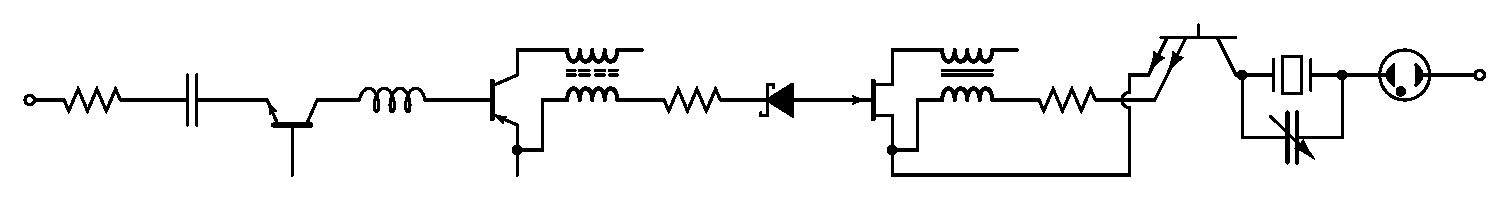
\includegraphics[width=\textwidth]{titlepage/border}
\end{minipage}

\vspace{-1in}
\vspace*{\fill}
\begin{center}
{\LARGE\@title}

\vspace{10mm}

\url{http://c4757p.com/projects/ps1}

\end{center}
\vspace*{\fill}

\vspace{-1in}
\begin{minipage}[c][1in][c]{\textwidth}
\begin{center}
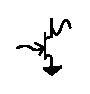
\includegraphics[width=20mm]{titlepage/logo} \\
\textcopyright ~\the\year ~\@author.
\end{center}
\end{minipage}

\makeatother

\end{titlepage}



\chapter{Specifications}
The PS-1 can be built in two versions, according to builder preference. The
PS-1H has a higher output voltage, but lower current. If you received a kit
including all parts, you must build the provided version.

Usually, the kit builder will select a mains transformer, so the input voltage
tolerance is unspecified. It will be determined by the properties of the
transformer.

\vspace{25mm}

\begin{center}
\begin{tabular}{|c|c|c|c|c|c|c|c|}
    \hline
    \multirow{2}{*}{\sc Model} & \multicolumn{2}{|c|}{\sc Output}
        & \multicolumn{2}{|c|}{\sc Regulation}
        & \multirow{2}{*}{\begin{minipage}[c]{1.5cm} \centering \sc Recov. time\end{minipage}}
    & \multicolumn{2}{|c|}{\sc Noise} \\ \cline{2-5} \cline{7-8}
        & \sc V & \sc mA & \sc Line & \sc Load & & \sc 0.1 -- 10~Hz & \sc 25 -- 2k~ Hz\\ \hline
    \hline

    PS-1H & 0--30~V & 0--500~mA & 0.01~\% & 0.01~\% & 100~$\mu$s &
        $<$ 500~$\mu $V$_{p-p}$ & $<$ 200~$\mu $V$_{PP}$ \\ \hline

    PS-1L & 0--18~V & 0--800~mA & 0.01~\% & 0.01~\% & 100~$\mu$s &
        $<$ 500~$\mu $V$_{p-p}$ & $<$ 200~$\mu $V$_{PP}$ \\ \hline

\end{tabular}

\ \\
Specifications valid over operating temperature range: 5--45~\dg C $\approx$ 40--110~\dg F.
\end{center}

Both PS-1H and PS-1L can withstand overloads of up to 200~V in either polarity
whether or not the unit is powered, and up to 45~V forward without blowing the
output fuse. Any reverse voltage above -0.7~V will blow the output fuse.

Note that schematics in this manual are drawn assuming the PS-1H model. The
principle of operation is identical for the PS-1L.


\tableofcontents

\mainmatter

\chapter{Introduction}
The PS-1 is a bench power supply intended for powering general analog and
digital devices under test (DUTs). It is designed entirely using
discrete semiconductors, and is designed to be as usable as a traditional power
supply based on precision operational amplifiers.

\subsubsection{Assembly}
To assemble the PS-1, you must handle and solder modern, surface-mount
devices (SMD). This manual will not teach you how to do this. A good
resource for learning how to solder SMD parts is the excellent soldering
video tutorial series by Dave Jones of EEVblog, which can be found on
YouTube:

\begin{center}
\begin{tabular}{lc}
\#180 --- Soldering Tutorial Part 1 --- Tools &
    \url{http://www.youtube.com/watch?v=J5Sb21qbpEQ} \\
\#183 --- Soldering Tutorial Part 2 &
    \url{http://www.youtube.com/watch?v=fYz5nIHH0iY} \\
\#186 --- Soldering Tutorial Part 3 --- Surface Mount &
    \url{http://www.youtube.com/watch?v=b9FC9fAlfQE} \\
\end{tabular}
{\small\it Please support Dave by disabling any ad blockers while watching
    these videos. This is how he makes his living.}
\hrule
\end{center}

You also may need to source the components to build the kit, as not all
incarnations provide all of the parts. A separate packet detailing parts which
were included and parts which were not should be attached; this will include
bills of materials (BOMs) directly compatible with multiple major parts
distributors to ease the process.

\subsubsection{Testing}
Testing the PS-1 requires only a multimeter of any kind and an oscilloscope
with at least 10 MHz bandwidth%
\footnote{Measuring some parameters requires more sophisticated equipment, but
I have done this already. If you build the PS-1 using the specified parts in
the specified manner, and you test it and find that it works, it should meet
these specifications.}.
You will build the supply one section at a
time, testing each individually, to isolate any problems to the exact section
which causes them. There is a troubleshooting guide in this booklet, but if you
encounter serious difficulty, you will find it necessary to read and understand
the Theory of Operation to fully debug the circuits.

\subsubsection{Voltage Warning!}
The ``low-voltage'' circuitry of this power supply contains voltages
ranging from 40~V to 50~V, which will probably not kill you, but could be
dangerous.  Do not touch the circuit while it is operational, and do not touch
anything powered by it until you have fully verified correct operation. You
should take care to fully determine and understand the paths by which dangerous
current can flow.

Assembling the PS-1 also requires you to make a small number of connections
that will operate at line voltage (120~V or 240~V AC, depending on your
country). It is \emph{your responsibility} to determine whether you can legally
perform this in your area, as I cannot be expected to know the electrical laws
of every jurisdiction. If this is prohibited or discouraged where you live,
I recommend finding someone licensed to do this wiring. Even if you \emph{can}
legally do this, I recommend politely asking someone with electrical experience
to check your work for safety.

\subsubsection{Energy Warning!}
Installing electrolytic capacitors backwards can make them \emph{pop!} If they
do this while your curious face is hovering over them, trying to figure out why
they are inflating like balloons, they can cause you physical injury. Any build
sections with capacitors in high-energy positions will advise you of this fact
before you power on the PS-1 for testing. I highly recommend covering the PS-1
and keeping your face away from it while connecting the power.

Likewise, resistors in any section of the circuit may burn if installed
incorrectly. This does not cause such a commotion as do the capacitors, but
it does smell very bad. You have been warned.


\chapter{Theory of Operation}
\section{Summary}

\begin{figure}[H]
\centering
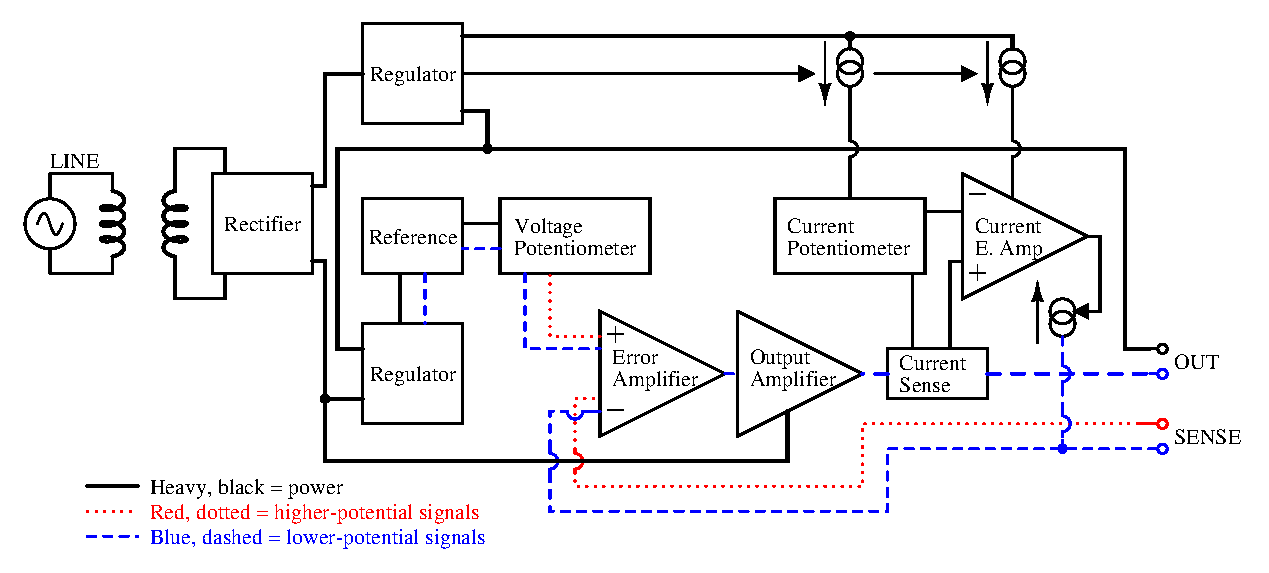
\includegraphics[width=5.5in]{sch/blockdiag}
\caption{Block diagram.}
\label{fig:blockdiag}
\end{figure}

\begin{multicols}{2}

Figure~\ref{fig:blockdiag} is the block diagram of the entire power supply.

First, the line (mains) voltage feeds the primary winding of a transformer,
giving approximately 28~VAC on the secondary.
This is rectified and filtered to DC by diode bridge \texttt{D1} and
capacitor \texttt{C1}.

The current exiting the rectifier passes through a simple ``regulator'',
consisting of just three diodes, to provide a pair of supply rails for
biasing current sources. To maintain good line regulation, the remaining
voltage feeds into a local regulator, giving a rail of approximately -32~V
to power the control circuitry.

This regulated rail powers a Zener reference diode. This regulates the
potential across the front-panel Voltage potentiometer, which is used to select
an output set-point.

The voltage from this potentiometer, as a differential pair, feeds into the
error amplifier, which compares it to the voltage sensed at the output, also as
a differential pair. If the relative voltage between the output pairs is above
that of the set-point, the output drive will be increased; if it is below, the
output drive will be decreased. The output will thus settle to almost exactly
the set-point.

After power leaves the output amplifier, it passes through a current sense
resistor. This resistor sees a potential difference, by Ohm's Law,
corresponding to the current flowing through it. A current sense amplifier
compares this to a current limit set-point; if the current drawn begins to
exceed the set level, the current sense amplifier will pull the negative sense
line further negative.  This causes the voltage amplifier to ``see'' too much
potential on the output, and it decreases output drive.


\end{multicols}

\section{Local Regulation}

To maintain good line regulation, the circuitry of the power supply is itself
powered by a local regulator.

\begin{figure}[H]
\centering
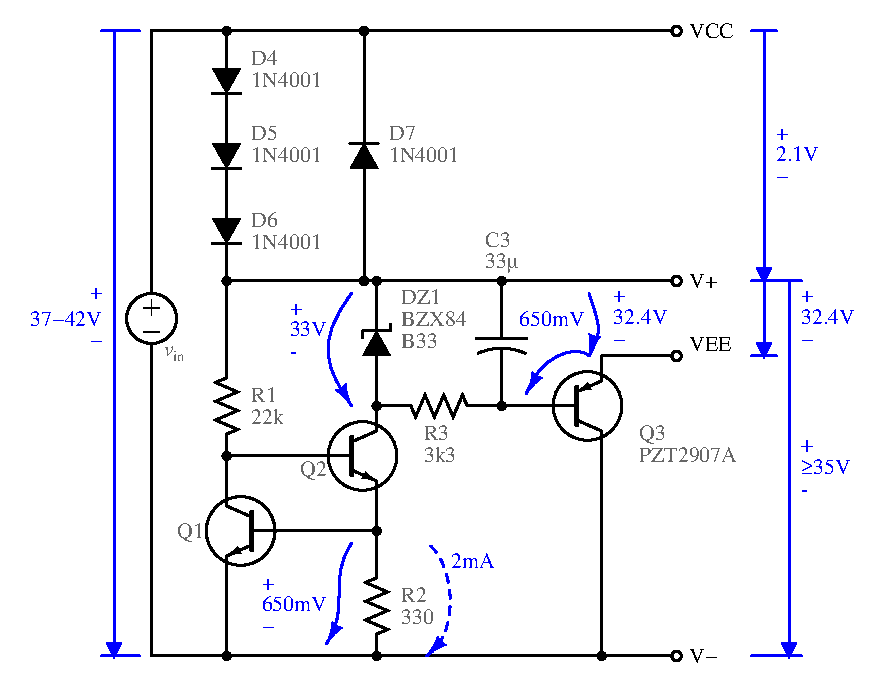
\includegraphics[width=5.5in]{sch/localregs}
\caption{Local regulator sub-schematic}
\label{fig:localreg}
\end{figure}

\begin{multicols}{2}

Note that unlike many electronic designs, this power supply uses a
\emph{positive ground} configuration. This means that rather than having
a higher voltage rail regulated with respect to a lower rail, the lower rail
is regulated to the higher one.

\subsubsection{VCC/V+ Auxiliary Rail}
A small positive rail is required about 2~V above ground to provide extra
headroom for the regulating circuits. The low current (500~mA) output means
that it is reasonably efficient to achieve this by passing the positive
supply input through a string of three diodes (0.7~V each, 2.1~V total), and
using the voltage appearing at the negative end as `ground', labeled V+ in the
circuit diagrams.
The voltage at the positive end is VCC.

This simple three-diode chain could barely be given the title ``voltage
regulator'', but it is used for this purpose.
Diode \texttt{D7}, connected backwards across the chain, protects the power
supply if an external voltage is applied to it while it is shut down. This
diode allows that external voltage to actually power the regulation circuitry,
protecting it from damage by reverse voltages.
\ \\

\subsubsection{VEE/V+ Primary Rail - Reference}
The VEE regulator is more complicated.

\texttt{Q1} and \texttt{Q2} act as a simple constant current source.
Consider what will happen
as the circuit starts up. The power switch will have just been flipped, and the
rails, once all equal in voltage, begin to drift apart.
\texttt{Q1} has \texttt{R2} pulling its base and
emitter together, so it begins turned off, and we can ignore it.
\texttt{Q2} has \texttt{R1} supplying it base current from V+, so it will
turn on. As V+ climbs, so does the current flowing through \texttt{Q2}, and
this same current flows through \texttt{R2}. Ohm's Law gives the voltage
across this resistor as equal to the product of the current and the resistance.
A typical transistor's threshold voltage is 650~mV. At this voltage, there is
$\frac{V}{R} = \frac{650\;mV}{330\;\Omega} = 1.97\;mA$ flowing. Because the
threshold voltage has been reached between \textrm{Q1}'s base and emitter,
\textrm{Q1} begins to turn on, diverting away \textrm{Q2}'s base current and
limiting the output current. This feedback action causes the current drawn
into \texttt{Q2} to settle at 1.97~mA.

\subsubsection{Primary Rail Regulation Tolerance}
Both the nominal 650~mV threshold voltage and the 330~$\Omega$ resistance
vary with temperature. The specified operating range of this power supply
is from 5~\dg C to 45~\dg C. The transistor's threshold voltage loses about
2~mV for every 1~\dg C above a standard 25~\dg C room temperature. 
A typical resistor might have a temperature coefficient of 200~ppm/\dg C,
or more properly, 200~($\mu\Omega$/$\Omega$)/\dg C,
meaning its resistance changes by 200~$\mu\Omega$ for every 1~$\Omega$
of its nominal value per 1~\dg C above the standard 25~\dg C.
This means that, assuming the threshold is indeed 650~mV at room temperature,
the temperature-dependent current drawn is:
\small
\begin{align*}
    & \textrm{Where } \Delta T = T - 25\;^\circ C\\
    &I(\Delta T) = \frac{V(\Delta T)}{R(\Delta T)} \\
    &\quad= \frac{650\;mV - (2\;mV/^\circ C)(\Delta T)}
      {(330\;\Omega)((200\;\mu\Omega/\Omega/^\circ C)(\Delta T) + 1)} \\
\end{align*}
\normalsize

This has its maximum value at the minimum value of $\Delta T$:
\small
\begin{align*}
    &I(-20^\circ C) = \frac{690\;mV}{328.68\;\Omega} = 2.10\;mA \\
\end{align*}
\normalsize

The error is $2.10\;mA - 1.97\;mA = 130\;\mu A$.

This 2~mA is drawn through \texttt{DZ1}, a BZX84-series, 2~\%-tolerance, 33~V
Zener diode, and this is precisely the current specified for the 2~\% tolerance.
The dynamic impedance (apparent output resistance at a specific bias point) of
\texttt{DZ1} is specified by the datasheet to be at worst 80~$\Omega$,
so the above
130~$\mu$A current error will cause a voltage error up to the product of the
two values:
$(130~\mu A)(80\;\Omega) = 10.4\;mV$, or 0.03~\% on top of the existing
2~\% tolerance. Further
error will be caused by \texttt{DZ1}'s temperature coefficient, given as
800ppm/\dg C: 1.6~\% in either direction over the specified range.
Assuming the temperature change is not enough to affect the dynamic
impedance, the errors can be added together, so
the total
non-trimmable voltage error is 1.6~\% + 0.03~\% = 1.63~\%. (The 2~\% is not
considered because it is constant --- a property of the individual diode ---
and can be adjusted with a trimmer).

\subsubsection{Primary Rail - Filter and Buffer}

The output voltage is filtered by \texttt{R3} and \texttt{C3}, a first-order
low pass filter with a cutoff frequency
$f_c = 1/(2\pi R_3 C_3) = 1.46\;Hz$ to filter out line ripple.
This is then buffered by \texttt{Q3}, a simple emitter-follower,
which loses about 650~mV: from -33~V to -32.35~V. It will have a 2~mV/\dg C
error just like \texttt{Q1}, contributing an additional 0.1~\% error, for a
grand total of 3.73~\%. There will be a slight, additional error in this
650~mV caused by self-heating and by load current, but this error is nearly
constant and will be calibrated away by the trimmers.

\end{multicols}

\section{Voltage Reference}

\begin{figure}[H]
\centering
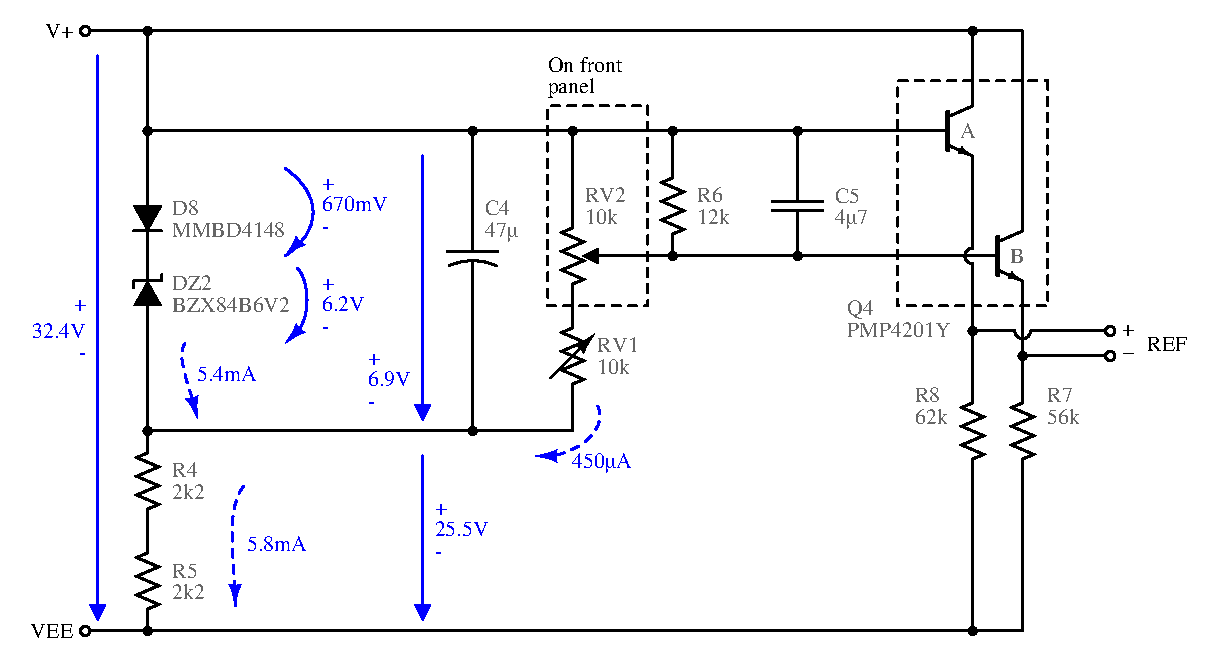
\includegraphics[width=5.5in]{sch/reference}
\caption{Voltage reference sub-schematic}
\label{fig:reference}
\end{figure}

\begin{multicols}{2}
To allow the power supply to output a fixed voltage, a voltage reference
circuit is used. This is essentially a second regulator, and because it is
run from the main regulator, the input power rejection compounds with that
of the main regulator.

\subsubsection{Reference Diode}
Zener diode \texttt{DZ2}, another BZX84-series 2~\% reference diode, is combined
with a standard MMBD4148 (surface-mount equivalent to the well known 1N4148)
in a sort of compound diode. The reason for this is temperature coefficients:
\end{multicols}

\begin{table}[H]
\centering
\begin{tabular}{l|llll}
 & & \multicolumn{3}{c}{Temperature error, mV/\dg C} \\
Diode & Voltage at 5~mA bias & (min) & (typ) & (max) \\
\hline
MMBD4148 & 670~mV & & -2 & \\
BZX84B6V2 & 6.2~V & 0.4 & 2.3 & 2.7 \\
\hline
Total & 6.87~V & -1.6 & 0.3 & 0.7 \\
\end{tabular}
\end{table}


\begin{multicols}{2}
Note that temperature coefficient of standard silicon PN diodes like the 4148
is much more regular, so only a `typical' value was given. This combination
gives a compound diode with a typical variation of only 0.3~mV/\dg C, or
0.09~\% over the full temperature range.

\subsubsection{Biasing}
Because only a pair of resistors (a pair, rather than just one, to share heat,
as they will get warm) is being used to supply current, there will be another
contribution to the error from the variation in VEE, calculated above. VEE can
have a drift-related (non-trimmable) error of up to 1.63~\%. This translates to
a variation in current through \texttt{R4} and \texttt{R5} of
$(0.0163)(32.4\;V-6.9\;V)/(4.4\;k\Omega) = 94.5\;\mu A$ in
either direction. The dynamic impedance of the BZX84B6V2, listed in the
datasheet, is no more than 10~$\Omega$. The dynamic impedance of the MMBD4148
is about 20~$\Omega$, which is not listed and must be measured from the
``Forward Voltage vs. Forward Current'' plot. This gives an error of up to
$(94.5\;\mu A)(30\;\Omega) = 2.84\;mV$ total, or 0.04~\%. Assuming the two
errors are not large enough to meaningfully affect each other, the total
non-trimmable error of the primary
reference is 0.13~\%.

\subsubsection{Potentiometer}
This reference voltage goes into front panel potentiometer \texttt{RV2}, and
a section of the voltage is trimmed off by \texttt{RV1} to compensate for
aforementioned variations in parts. \texttt{R6} ensures that if \texttt{RV2}'s
wiper becomes disconnected (a somewhat common failure mode in panel-type
potentiometers), the output voltage defaults to zero. \texttt{C5} provides
extra filtering to remove any noise picked up by the cable running to the
panel.

\subsubsection{Output Buffer}
\texttt{Q4} is a pair of NPN transistors, factory-selected to have nearly
identical
characteristics and mounted in one small package to ensure equal temperature.
Each transistor is used to buffer one side of the reference voltage, and
despite the approximately 650~mV drop, the relative voltage should still be
equal because of the matched characteristics. Buffering is necessary because
the error amplifier requires a known impedance of the input signals, but the
impedance at the output of a potentiometer changes drastically over the
range. The output impedance of an emitter follower is very low, and will be
dominated by the resistors in the error amplifier.

\texttt{R7} and \texttt{R8} are selected to give as close to equal currents
through each half of \texttt{Q4} as possible, without using an active current
source circuit. Using V+ as a reference ground for calculation, \texttt{Q4A}
will always see 0~V on its base, and so its emitter will give -0.65~V.
With VEE as -32.4~V, \texttt{R8} will see 31.75~V, drawing 512~$\mu$A.
As the potentiometer is turned, the voltage at \texttt{Q4B}'s base and emitter
will change, ranging from -0.65~V at the emitter to -5.30~V. This gives a
current range through \texttt{R7} from 484~$\mu$A to 567~$\mu$A, centered
at  525~$\mu$A.

\end{multicols}

\section{Voltage Error Amplifier}

\begin{figure}[H]
\centering
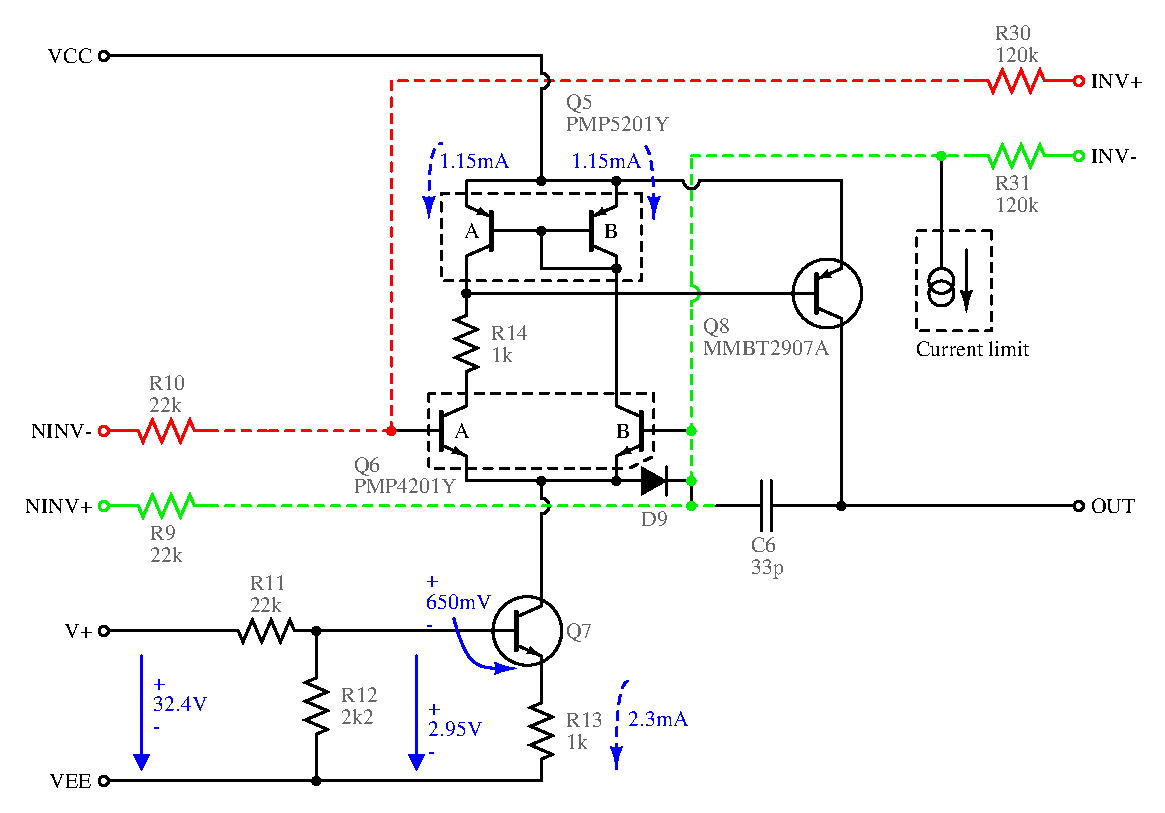
\includegraphics[width=5.5in]{sch/verror}
\caption{Voltage error amplifier sub-schematic}
\label{fig:verror}
\end{figure}

\begin{multicols}{2}

An error amplifier is a circuit which compares a reference level to the
actual output, adjusting the output driver according to the amount of error
present. This is done simply by subtracting the output level from the
reference level, amplifying the difference by a large amount, and using
this directly to control the output.

The error amplifier shown above is based on a transistor arrangement
called a ``long-tailed
pair'' or ``differential pair'' (Fig. \ref{fig:ltp}). This is the heart of
most differential circuits, including the operational amplifier.


\begin{figure}[H]
\centering
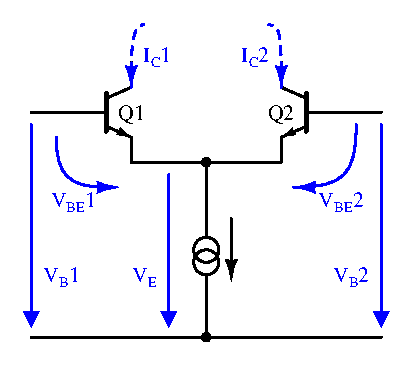
\includegraphics[width=2in]{sch/ltp}
\caption{Long-tailed pair}
\label{fig:ltp}
\end{figure}

\subsubsection{Long-Tailed Pair}
I will spare you the mathematics of fully analyzing the long-tailed pair,
because it is very easy to explain without numbers. Imagine the saturated
case. This is where the two input voltages, $V_{BE}1$ and $V_{BE}2$, are
vastly different, so the output is as large as it possibly can be. Suppose
$V_{BE}2$ is significantly greater than $V_{BE}1$. The voltage at the
emitters, $V_E$, must be one B-E drop less than $V_{BE}2$. This is because if
it were any lower, \texttt{Q2}'s B-E diode would be forward biased, and would
begin to conduct. So \texttt{Q2} will be conducting, with $I_C2 > 0$, and
\texttt{Q1} will not conduct, with $I_C1 = 0$, because its B-E diode will not
be forward biased. Therefore, the current draw into the transistors is
determined by which of the two voltages is larger. This is a comparator.

If $V_B1$ and $V_B2$ are very close, both transistors will conduct, with
the one having a larger $V_{BE}$ conducting more. $V_E$ will be determined
by both base voltages, and since $V_{BE}$ is just $V_B - V_E$, the current
into each transistor will be determined by the \emph{relative} voltage
between the bases. This is a proper differential amplifier.

\subsubsection{Sources of Error}
The voltage error amplifier must be a \emph{precision} amplifier. 
A matched pair, \texttt{Q6}, is used, to make sure the gains and
threshold voltages on each side are the same. Still, there is more variation
that must be corrected. First, if the two transistors draw significantly
different currents, their gains and thresholds change. \texttt{Q5} is another
matched pair, acting as a current mirror. \texttt{Q5B} is diode-connected,
so that current may be drawn through it, and \texttt{Q5A} is
transistor-connected to the same $V_{BE}$, so that it will pass the same
current. This stabilizes the current difference between the two, and
\texttt{Q7}, a simple current source, stabilizes the total current.

An error amplifier must have extremely high gain in order to be precise.
This is because its operation \emph{depends} on a small error being present.
Higher gain means it will be sensitive to a smaller error.
\texttt{Q8} is connected as a simple common-emitter amplifier
to provide voltage gain to the output.

\subsubsection{Feedback Mechanism}
Feedback paths are colored in Figure \ref{fig:verror}. 
{\small \it Note: If you are reading a
greyscale copy, the paths have been marked with dashed lines; the red path
lies on top and runs through \texttt{R10}, and the green path lies underneath
and runs through \texttt{R9}.}
The red path is
noninverting: if the voltage on that path is increased, the voltage on
\texttt{Q8}'s collector (the output) will also increase. The green path
is inverting. As an example of the corrective action of the circuit: Imagine
that there
is voltage loss in the positive output lead's resistance.
The noninverting path will fall (as the positive output lead is connected
to ``INV+''),
and ``OUT'', which drives the \emph{negative}
output lead, will fall in turn. The overall output voltage will increase,
compensating for the drop in the positive lead.

\texttt{C6} exists to slow down the error amplifier. If the output drops
too quickly, \texttt{C6} will begin to conduct, pulling down the inverting
path, and therefore pulling the output back up. This is necessary for
stability. Without it, the error amplifier can operate faster than the
lag of the feedback system, causing it to ``see'' a delayed reading and
leading to oscillation.

\subsubsection{External Cutoffs}
Both the current limiter and the thermal cutoff shut down the output by
pulling the inverting path down (thus pulling the negative output up). If the
path is pulled below the emitter voltage of \texttt{Q6}, \texttt{Q6B}'s B-E
junction will be reverse biased, which can cause damage. \texttt{D9} limits
this reverse bias to -0.7\;V. Unfortunately, this provides a path for
unlimited current (through \texttt{Q8} E-B, then through \texttt{Q6A} C-E,
then through \texttt{D9}), so \texttt{R14} is installed to limit the current.

\end{multicols}

\section{Current Error Amplifier}

\begin{figure}[H]
\centering
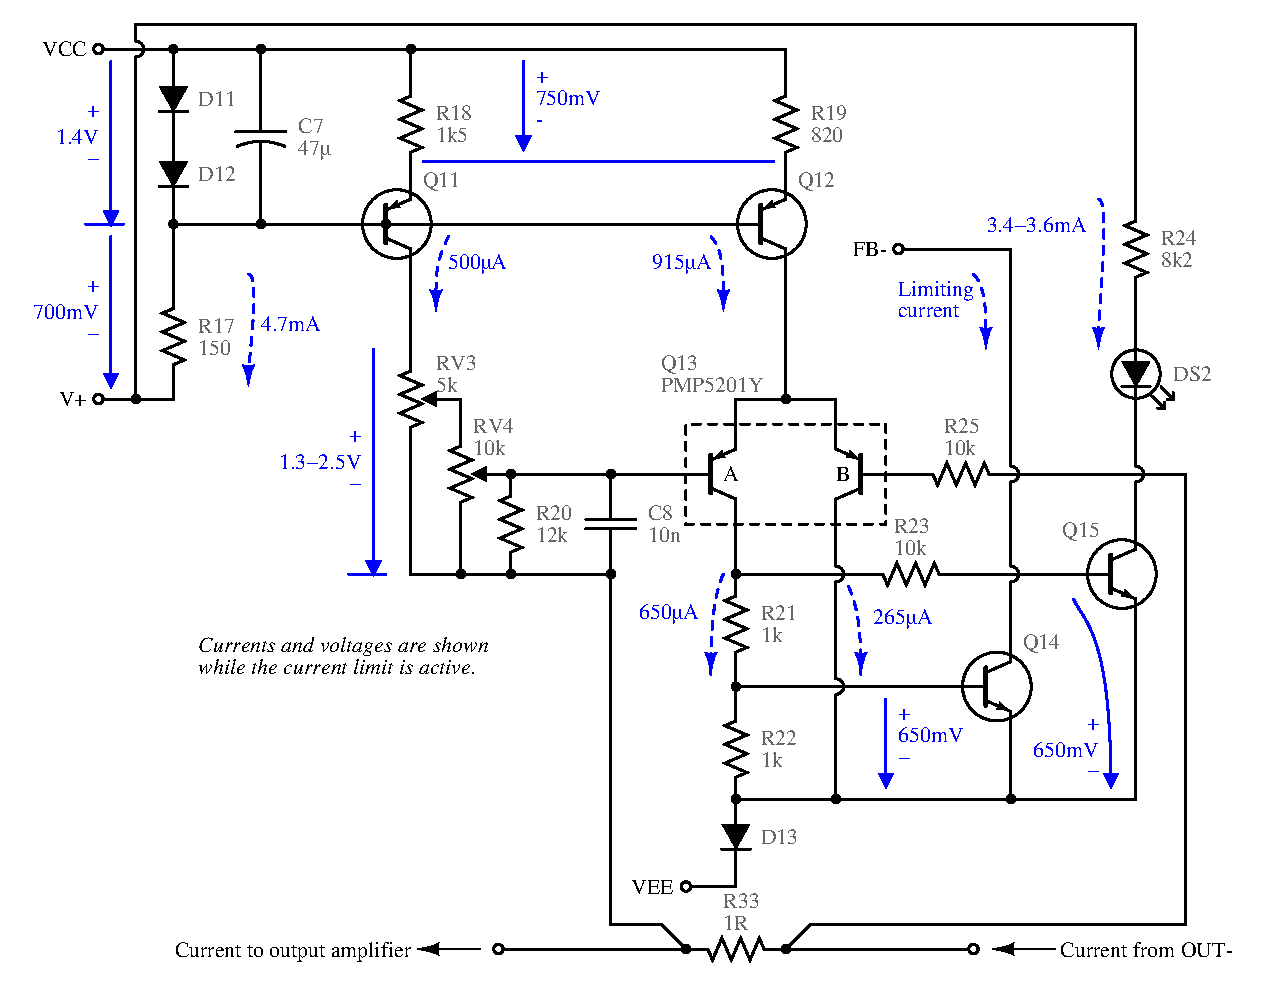
\includegraphics[width=5.5in]{sch/ierror}
\caption{Current error amplifier sub-schematic}
\label{fig:ierror}
\end{figure}

\begin{multicols}{2}

The current error amplifier is similar. The output current $I$ passes through a
1~$\Omega$ resistor, \texttt{R33}, which causes a drop by Ohm's law of $V =
I(1\;\Omega)$. (Note that because the sense lines connect on the output side
of \texttt{R33}, they cancel this drop at the output.) Another long-tailed pair
compares this drop to a reference level.

\subsubsection{Reference}
\texttt{D11} and \texttt{D12} establish a 1.4\;V reference voltage, in the same
way as \texttt{D4}, \texttt{D5} and \texttt{D6} (Fig. \ref{fig:localreg}). The
reason two separate diodes are used, rather than simply using the voltage
between \texttt{D4} and \texttt{D5}, is that the output current itself passes
through \texttt{D4} and \texttt{D5}. This would be a source of error, causing
the current limit to increase as the output current increased. This positive
feedback could lead to oscillation, and would certainly at least lead to an
incorrect limit level.

\subsubsection{Biasing and Potentiometer}
This reference controls two current sources, \texttt{Q11} and \texttt{Q12}, in
the same way as \texttt{Q7} in the voltage error amplifier (Fig.
\ref{fig:verror}). The current through \texttt{Q11} feeds into \texttt{RV3},
which then goes to the inner side of \texttt{R33}. Because the current is
constant, \texttt{RV3} experiences a constant Ohmic voltage drop, and the
bottom end of \texttt{RV3} is fixed at the same voltage as the inner side
of \texttt{R33}. \texttt{RV3} is trimmed to set the highest current limit,
and \texttt{RV4} sits on the front panel, allowing the output current limit to
be set. In the same function as \texttt{R6} (Fig. \ref{fig:reference}),
\texttt{R20} ensures that the current limit defaults low if the current control
potentiometer is disconnected or damaged.

\subsubsection{Limiting Action}
When the current reaches the limit value, the voltage on the outer side of
\texttt{R33} will be equal to the voltage at the output of \texttt{RV4}.
The voltage on \texttt{Q13B}'s base will rise towards its emitter, and it will
stop conducting. At the same time, \texttt{Q13A} will begin conducting. The
current through it flows through \texttt{R22}, causing a voltage drop which
activates \texttt{Q14}, pulling down the inverting feedback line and dropping
the output voltage.

The same current flows through \texttt{R21}, causing another voltage drop,
which is applied to \texttt{Q15}'s base. This turns on LED \texttt{DS2},
indicating to the operator that the current limit is active.

\texttt{C8} fulfills a similar purpose to \texttt{C6} in the voltage error
amplifier (Fig. \ref{fig:verror}): compensating for feedback lags to stabilize
the amplifier. At the same time, it fulfills the same purpose as \texttt{C5} in
the voltage reference (Fig. \ref{fig:reference}), shunting away any
electromagnetic interference picked up by the cable to the panel.

\subsubsection{Protection}
\texttt{R25} protects \texttt{Q13B} from a sudden voltage spike if the output
is shorted or a voltage is applied to it. If a voltage greater than 32.4\;V
is applied to the output,
\texttt{Q13B} would be reverse-biased from
OUT- to VEE; \texttt{D13} protects it from this.

\end{multicols}

\section{Thermal Cutoff}

\begin{multicols}{2}

\begin{figure}[H]
\centering
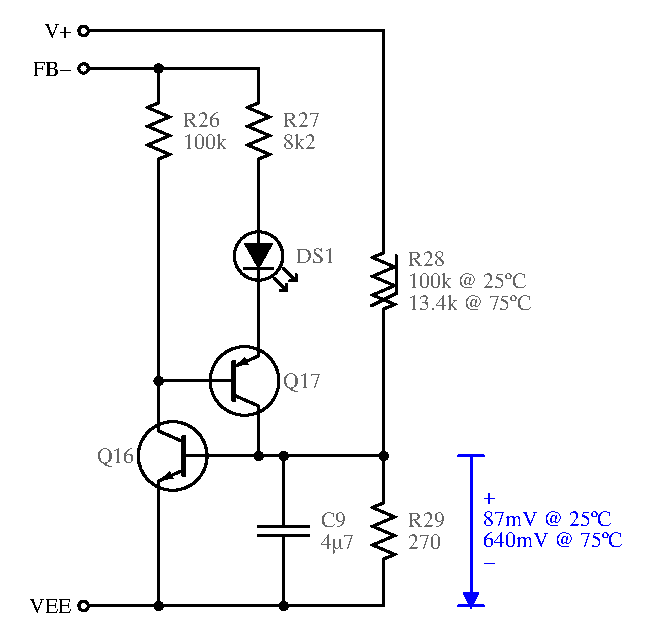
\includegraphics[width=3in]{sch/thermal}
\caption{Thermal cutoff sub-schematic}
\label{fig:thermal}
\end{figure}

The thermal cutoff circuit almost entirely comprises a simulated thyristor,
made from a pair of bipolar transistors.

\begin{figure}[H]
\centering
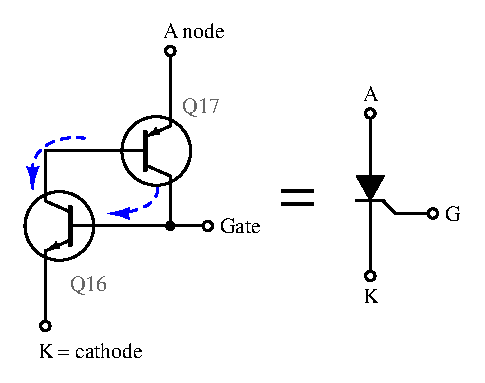
\includegraphics[width=\columnwidth]{sch/thy}
\caption{Simulated thyristor}
\label{fig:thy}
\end{figure}

\subsubsection{Thyristor}

A true thyristor is a device related to the bipolar transistor, made from
four alternating semiconductor layers, P-N-P-N, rather than three.
Unlike the bipolar transistor, it is \emph{bistable}. This means it has a
memory effect --- it can be either `on' or `off', and when put into one of
those states, it will remain there until switched again.

Most thyristors are \emph{silicon controlled rectifiers}, or SCRs.
The SCR's symbol looks like a diode with an extra lead, the \emph{gate}.
In its startup position, with the gate voltage near the cathode voltage, it
does not conduct in either direction. When the gate is activated like the base
of a bipolar transistor, the thyristor begins to act like a diode, conducting
forward. It will switch back off, and stay that way until triggered again, when
the current through it falls to zero or it is reverse-biased.

I have avoided the use of the term `SCR' here, because `rectifier' implies that
it can be usefully employed in positions where it will be reverse-biased, but
this two-transistor simulated thyristor will not tolerate reverse bias. It is
only useful in forward-bias-only situations.

\subsubsection{Simulated Thyristor}
When the simulated thyristor is powered on, and the gate voltage is near the
cathode voltage, neither transistor has a source for base current, so
neither transistor conducts. When the gate voltage is raised, and current flows
into the gate, \texttt{Q16} begins to conduct. When it does, it pulls its own
collector current, causing \texttt{Q17} to begin to conduct. \texttt{Q17}'s
collector current flows into \texttt{Q16}'s base, causing \texttt{Q16} to
continue to conduct. In this manner, each transistor keeps the other conducting
until no more current can flow, even if the external source of gate current is
removed.

\subsubsection{Thermistor}
A thermistor is a resistor with a temperature coefficient large enough, and
accurate enough, to be useful for temperature measurement. \texttt{R28} is
a negative temperature coefficient (NTC) thermistor with a resistance of
100~$k\Omega$ at a 25~\dg C room temperature, decreasing to 13.4~$k\Omega$
at 75~\dg C. This changes the bias point given by the \texttt{R28}%
/\texttt{R29} voltage divider. At 75~\dg C, the voltage applied to the
gate of the simulated thyristor is:

\begin{align*}
    &(V^+ - VEE)\frac{R29}{R29+R28} = (32.4\;V)\frac{270\;\Omega}{270\;\Omega + 13.4\;k\Omega} \\
    &\quad {}= 640\;mV
\end{align*}

This is near the point where the thyristor turns on.

\subsubsection{Limiting Action}
When the thyristor conducts, it conducts \emph{through} the negative feedback
path. The path is unimpeded except for \texttt{R14} (1\;$k\Omega$) once the
voltage error amplifier saturates, allowing a few milliamps to flow from VCC,
through \texttt{Q8} E-B, through \texttt{R14}, through \texttt{Q6A} C-E, through
\texttt{D9}, and to the thyristor. Pulling the feedback path down limits the
output current in the same way as \texttt{Q14} in the current error amplifier.
This current flows through \texttt{R27} and the LED \texttt{DS1}, causing it
to glow.

\end{multicols}

\section{Output Amplifier and Output}

\begin{figure}[H]
\centering
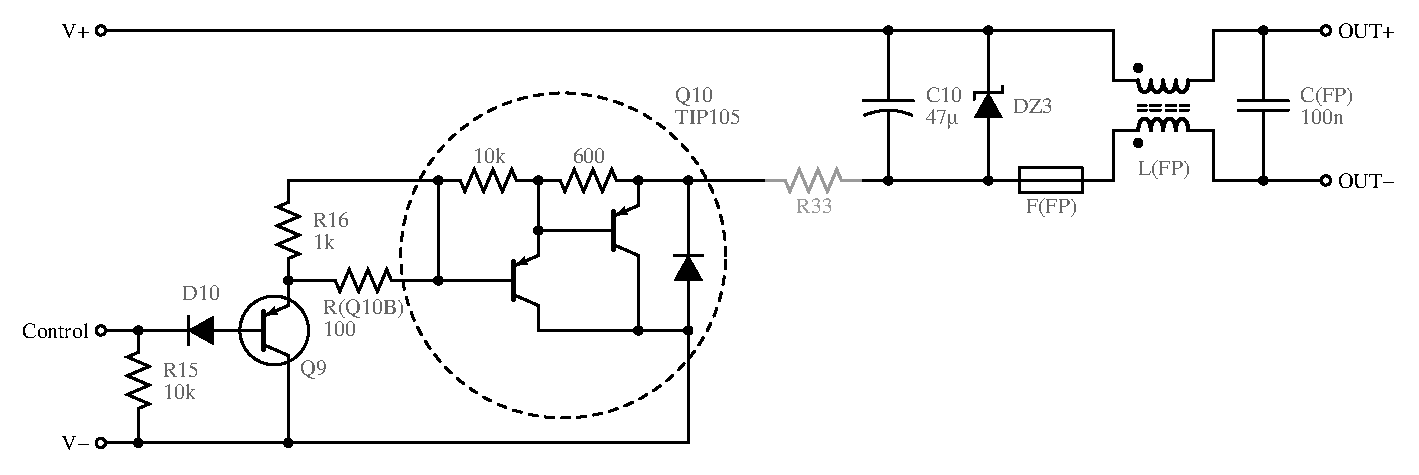
\includegraphics[width=5in]{sch/output}
\caption{Output sub-schematic}
\label{fig:output}
\end{figure}

\begin{multicols}{2}

The output amplifier buffers the signal from the voltage error amplifier, so
that it can supply the 500~mA output current. This is a simple circuit,
consisting of three emitter followers chained in a Darlington configuration.

The control signal is a current, not a voltage, so it is passed into
\texttt{R15} to convert it to voltage by Ohm's law. \texttt{D10} allows
current to sink out of \texttt{Q9}'s base, but prevents \texttt{Q9} from
being reverse-biased if a voltage is applied externally to the output.
\texttt{Q9} feeds \texttt{Q10}, which is a simple integrated circuit containing
two PNP transistors in a Darlington pair, the resistors connecting them, and a
diode from collector to emitter. This diode is also used for protection: if
a voltage is applied to the output while the PS-1 is unpowered, the diode will
allow this voltage to power the circuitry, developing proper bias voltages in
the system and protecting it from harm.

\texttt{C10} stores output charge, improving the transient response of the
power supply, and is also necessary for stability of the control loop.

\subsubsection{Parasitic Oscillators}
\texttt{R(Q10B)} is a ``base stopper'' resistor%
\footnote{If one wanted to research this topic further, one would find the
search term ``grid stopper'' more fruitful.}.
This resistor is installed directly at the base pin of \texttt{Q10}
(which is mounted off the board on wires). It forms an R-C low pass filter
with the tranistor's inherent base capacitance. This performs two functions.
First, it filters away any radio interference picked up by the wires, so that
this interference is not amplified and conducted to the output. Second, it
isolates the inductance of the wire from the transistor's base, preventing
an unintentional, parasitic Colpitts or Clapp oscillator from being formed from
the transistor and surrounding parasitics.

\subsubsection{Output Filter}
\texttt{L(FP)} and \texttt{C(FP)}, wired off-board, form a simple output
filter. This is not actually meant to filter the current on its way out, to
improve conditions for the DUT, but actually the reverse: if the DUT generates
any high-frequency currents, or if the test leads act as antennas and pick up
any high-frequency signals, they will block them from being absorbed by and
affecting the internal circuits. Capacitor \texttt{C(FP)} will shunt off any
differential currents from one wire to the other, and common-mode choke
\texttt{L(FP)} will block any common-mode (equal polarity in both wires)
currents.

\subsubsection{Output Protection}
In addition to the myriad small circuit additions (mostly diodes) already
described which protect the output in case of overload, there are two specific,
dedicated output protection devices.

\texttt{DZ3} is a transient voltage suppression (TVS) diode. In the PS-1H
model, it is a Vishay SMCJ30A. This is a form of Zener (actually avalanche)
diode, designed not to conduct at all up to 30~V, to begin conducting no higher
than 48.4~V, and to be able to withstand pulse currents of up to 31~A. Just
like a normal Zener diode, it will always conduct in the forward direction
(a negative voltage applied to the output) If an excessive voltage overload
applied, \texttt{DZ3} will crowbar it, blowing fuse \texttt{F(FP)} and
protecting the PS-1. The circuit is capable of directly withstanding overloads
up to this point without requiring the fuse to be blown.

\end{multicols}


%\begin{appendices}

%\chapter{Prototyping}
%\input{appendix-proto/appendix-proto}
%\end{appendices}

\end{document}
